%cSpell:disable
\subsection{Geodaten zu Hypotheken und Hochwasser}
\subsubsection{Hypothekengeodaten}\label{sec:hypogeo}

Für die Kompatibilität von Hypotheken- und Hochwasserdaten sind geografische Koordinaten erforderlich. Dieser Abschnitt befasst sich mit der Generierung präziser Koordinaten für die Datenpunkte.

Eine zufällige Verteilung in Bayern würde die Struktur eines Kreditportfolios nicht korrekt abbilden, da eine ungleichmäßige Verteilung von Immobilien sowohl in Deutschland als auch in Bayern zu beobachten ist. \textcite{zurek2022real} analysierte die Beziehung zwischen Bevölkerungsdichte und Kreditvergabe in Deutschland. Die Studie zeigt, dass Regionen mit stärkerem Wirtschaftswachstum höhere Immobilienpreise aufweisen. Dies führt zu einer erhöhten Kreditnachfrage. Auf Basis dieser empirischen Erkenntnisse wird die Bevölkerungsdichte als Grundlage für die Zuweisung spezifischer Koordinaten zu jedem Datenpunkt herangezogen.

Die verwendete Datenquelle stammt von \textcite{suche_postleitzahl}. Sie kombiniert OpenStreetMap-Daten mit Einwohnerzahlen von \textcite{destatis}. Dies ermöglicht eine präzise Segmentierung in Postleitzahlenzonen. Tabelle \ref{tab:geodaten} zeigt die Daten dieser geographischen Strukturierung.
Übersicht der Geodaten für Postleitzahlgebiete in Bayern
\begin{table}[htbp]
    \centering
    \small
    \caption{Übersicht der Geodaten für Postleitzahlgebiete in Bayern}
    \label{tab:geodaten}
    \begin{tabularx}{1.0\textwidth}{>{\raggedright\arraybackslash}X >{\raggedright\arraybackslash}X}
        \toprule
        \textbf{Objekt} & \textbf{Erklärung} \\
        \midrule
        plz & Postleitzahl \\
        \addlinespace
        einwohner & Die Einwohnerzahl eines bestimmten Ortes \\
        \addlinespace
        qkm & Die Fläche des Gebiets in Quadratkilometern \\
        \addlinespace
        geometry & Die Koordinaten des Gebiets \\
        \addlinespace
        ort & Der Name des Ortes, in dem sich das Gebiet befindet \\
        \addlinespace
        landkreis & Die Zugehörigkeit zu einem Landkreis \\
        \bottomrule
    \end{tabularx}
\end{table}
\FloatBarrier


Tabelle \ref{tab:geodaten} wurde aus Shapefile-Daten der Postleitzahlenregionen generiert und umfasst die Bevölkerungsverteilung. Vier Spalten sind von besonderer Relevanz: Ort, Landkreis, Geometrie und Einwohner. Die Geometriespalte enthält die geografischen Koordinaten der Gemeinden, dargestellt als Polygon oder Multipolygon. Ein Multipolygon setzt sich aus mehreren Einzelpolygonen verschiedener Formen zusammen. Zur räumlichen Referenzierung dient das Koordinatensystem EPSG:3035. Abbildung \ref{fig:bevoelkerungsdichte} visualisiert die aus diesen Daten abgeleitete Bevölkerungsdichteverteilung Bayerns nach Postleitzahlenbereichen.

\begin{figure}[htbp]
    \centering
    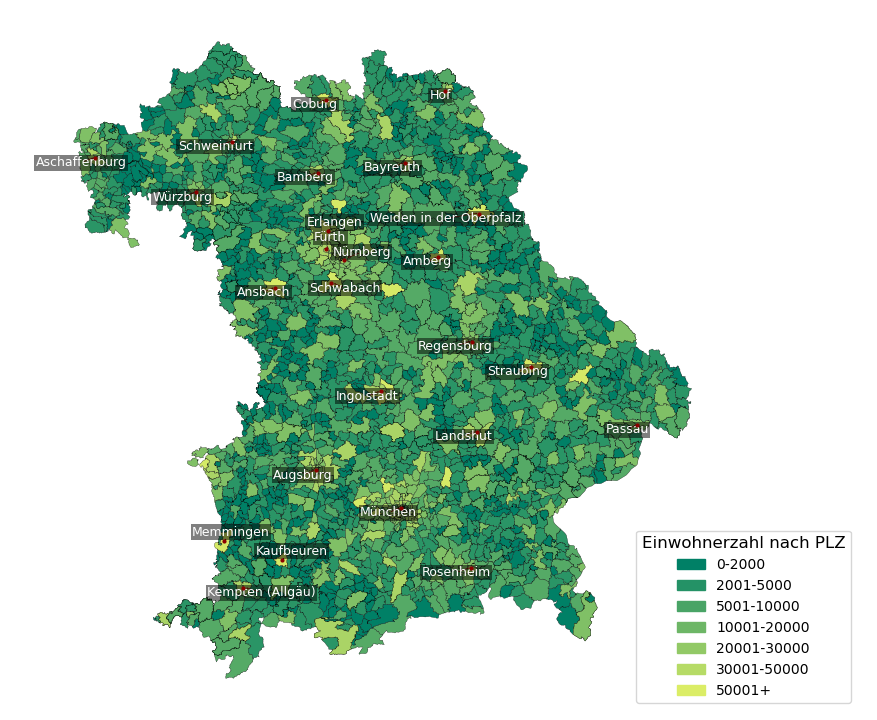
\includegraphics[width=0.95\textwidth]{figures/Bayern_pop_plz.png}
    \caption{Verteilung der Bevölkerungsdichte Bayerns nach Postleitzahlenbereichen. Quelle: Eigene Darstellung}
    \label{fig:bevoelkerungsdichte}
\end{figure}
\FloatBarrier

Zur repräsentativen Verteilung der 3853 Datenpunkte, entsprechend der Anzahl der Hypothekarkredite, wird ein proportionaler Ansatz implementiert, der auf der Einwohnerzahl jeder Region basiert. Innerhalb der Postleitzahlgebiete erfolgt die Platzierung mittels eines kontrollierten stochastischen Verfahrens. Für jede Region wird eine zuvor determinierte Anzahl von Zufallspunkten innerhalb der definierten Gebietsgrenzen generiert. Jedem Punkt werden spezifische Koordinaten in Form von Latitude (Breitengrad) und Longitude (Längengrad) zugewiesen. Anschließend wird eine Verifikation der Lage innerhalb des jeweiligen Polygons durchgeführt. Bei erfolgreicher Validierung wird der Punkt mit seinen Latitude- und Longitude-Koordinaten in die Liste der akzeptierten Datenpunkte integriert.Abbildung \ref{fig:hypothekenportfolio} zeigt die resultierende Distribution der Datenpunkte auf der Karte Bayerns.

\begin{figure}[htbp]
    \centering
    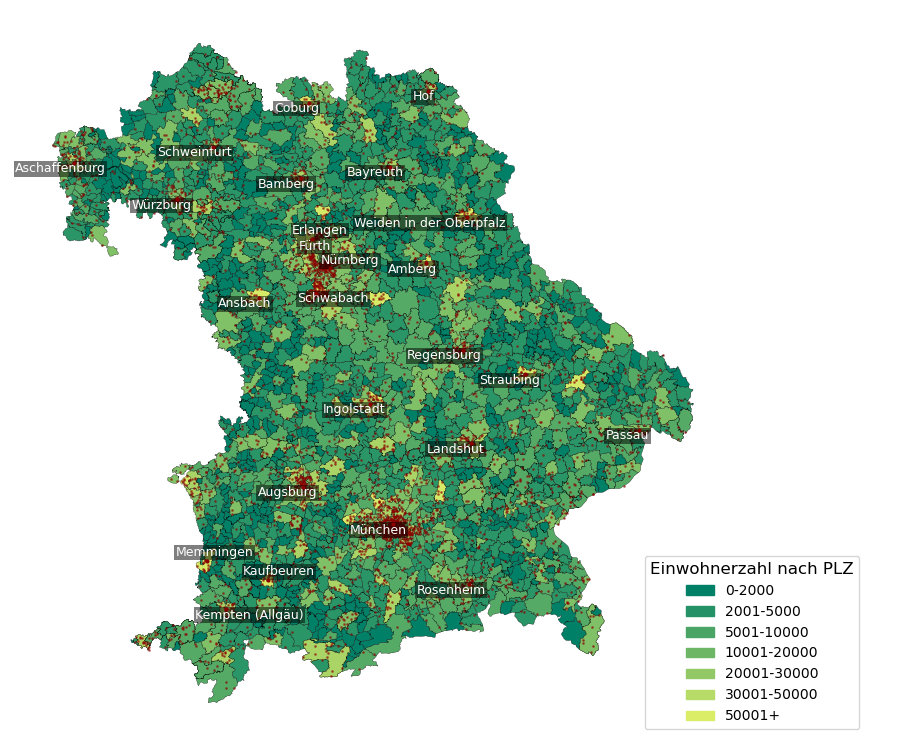
\includegraphics[width=\textwidth]{figures/bayern_por_pop.png} 
    \caption{Datenpunktverteilung im Hypothekenportfolio Bayern. Quelle: Eigene Darstellung}
    \label{fig:hypothekenportfolio}
\end{figure}
\FloatBarrier

\subsubsection{Hochwassergeodaten}\label{sec:hochgeo}

Im Anschluss an die in Abschnitt \ref{sec:hypogeo} dargelegte Erfassung der geografischen Koordinaten der Hypothekendarlehen ergibt sich die Notwendigkeit einer weiterführenden Analyse. Diese zielt darauf ab, die räumliche Relation der betreffenden Immobilien zu den definierten Hochwasserrisikogebieten zu determinieren. Zur Durchführung dieser Analyse ist eine detaillierte Hochwasserrisikokarte für Bayern erforderlich.

Im Rahmen eines EU-weiten Stresstests stellt die \ac{EZB} den Banken zur Simulation eines schweren Überschwemmungsszenarios eine Hochwasserrisikokarte (Abbildung \ref{fig:euflut}) zur Verfügung.

\begin{figure}[htbp]
    \centering
    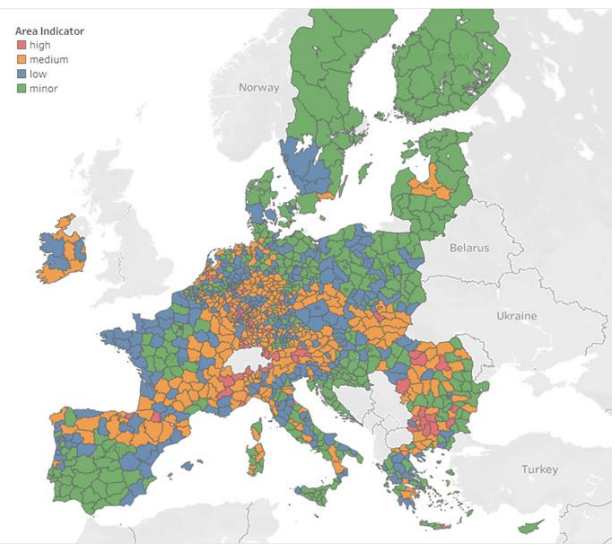
\includegraphics[width=0.6\textwidth]{figures/euflood.png} 
    \caption{EU-Hochwasserrisikokarte.Quelle: EZB 2022 Klimarisiko-Stresstest}
    \label{fig:euflut}
\end{figure}
\FloatBarrier

Die \ac{EZB}-Karte klassifiziert Regionen nach Hochwasserrisiken. Sie basiert auf Daten der Europäischen Kommission und Four Twenty Seven \parencite{ECB2022ClimateStressTest}. Allerdings sind die Basisdaten nicht öffentlich zugänglich. Zudem erlaubt die visuelle Darstellung keine präzise Identifikation spezifischer Gebiete. Folglich ergibt sich für Bayern die Notwendigkeit einer detaillierteren Analyse.

Die Kartierungen des Bayerischen Landesamts für Umwelt bieten eine fundierte Grundlage für die regionale Risikoanalyse. Diese für die Einzugsgebiete von Donau, Rhein und Elbe entwickelten Karten ermöglichen eine präzise Einschätzung der Hochwasserrisiken in Bayern \parencite{LfU_Bayern}. Sie visualisieren detailliert die Hochwassergefährdung, potenziell betroffene Landnutzungen und historische Hochwasserereignisse.
Diese Daten liegen aber im ETRS89-Koordinatensystem vor, während die Hypothekengeodaten das EPSG:3035-System nutzen. Zur Herstellung der Datenkohärenz erfolgt eine Koordinatentransformation in das EPSG:3035-System. Abbildung \ref{fig:bayernflut} präsentiert das Resultat dieser Vereinheitlichung und visualisiert die räumliche Verteilung der Hochwasserrisikogebiete Bayerns.
\begin{figure}[htbp]
    \centering
    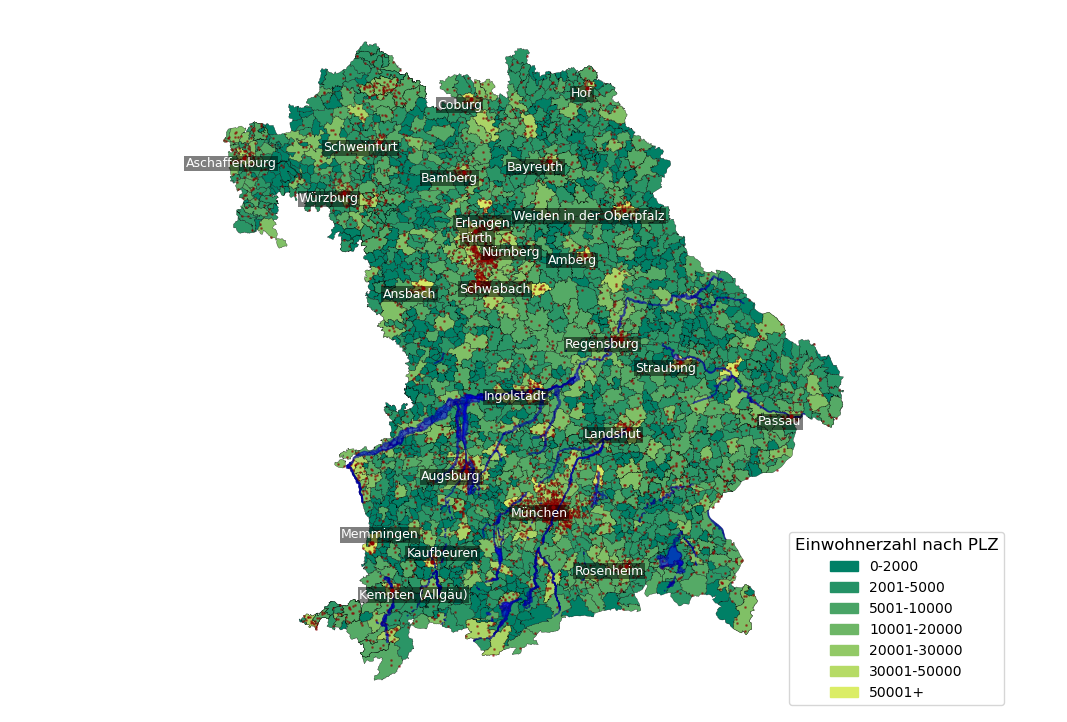
\includegraphics[width=\textwidth]{figures/bayern_flut.png} 
    \caption{Visualisierung historischer Hochwasserereignisgebiete und Verteilung des Darlehensportfolios in Bayern. Quelle: Eigene Darstellung}
    \label{fig:bayernflut}
\end{figure}
\FloatBarrier


\subsubsection{Überflutungstiefen}\label{sec:tief}
Die Schäden durch Überschwemmungen hängen von der Wassertiefe ab. Tieferes Wasser verursacht meist größere und teurere Schäden an Häusern. Für die Analyse der Überflutungstiefe in Bayern benötigt man Überflutungstiefen-Geodaten. \ac{DGM} Modell beschreibt die Höhe des Bodens, wobei eine hohe Auflösung genaue Ergebnisse liefert \parencite{vermessungsverwaltung2019gelandemodell}. Hochwasserstände aus Messungen sind wichtig für präzise Berechnungen. Dafür wurden Daten vom \textcite{bayern2016hochwassernachrichtendienst} für aktuelle Pegelstände betrachtet. Historische Hochwasserdaten helfen bei Einschätzungen künftiger Ereignisse und sind in Berichten und Karten enthalten. Diese wurden vom \textcite{LfU_Bayern} bezogen, wie in Abschnitt \ref{sec:hochgeo} beschrieben.
Die \ac{DGM}-Daten von \textcite{vermessungsverwaltung2019gelandemodell} für ganz Bayern umfassen ein sehr großes Datenvolumen von ca. 240 GB. Daher wurden nur Daten für die Gebiete mit Hypotheken-Datenpunkten aus Abschnitt \ref{sec:hypogeo} heruntergeladen. Abbildung \ref{fig:ingolstadt} visualisiert das digitale Geländemodell für Ingolstadt, welches die topographischen Merkmale der Stadt und ihrer Umgebung detailliert darstellt und somit eine wichtige Grundlage für die Hochwasseranalyse bildet.
\begin{figure}[!ht]
    \centering
    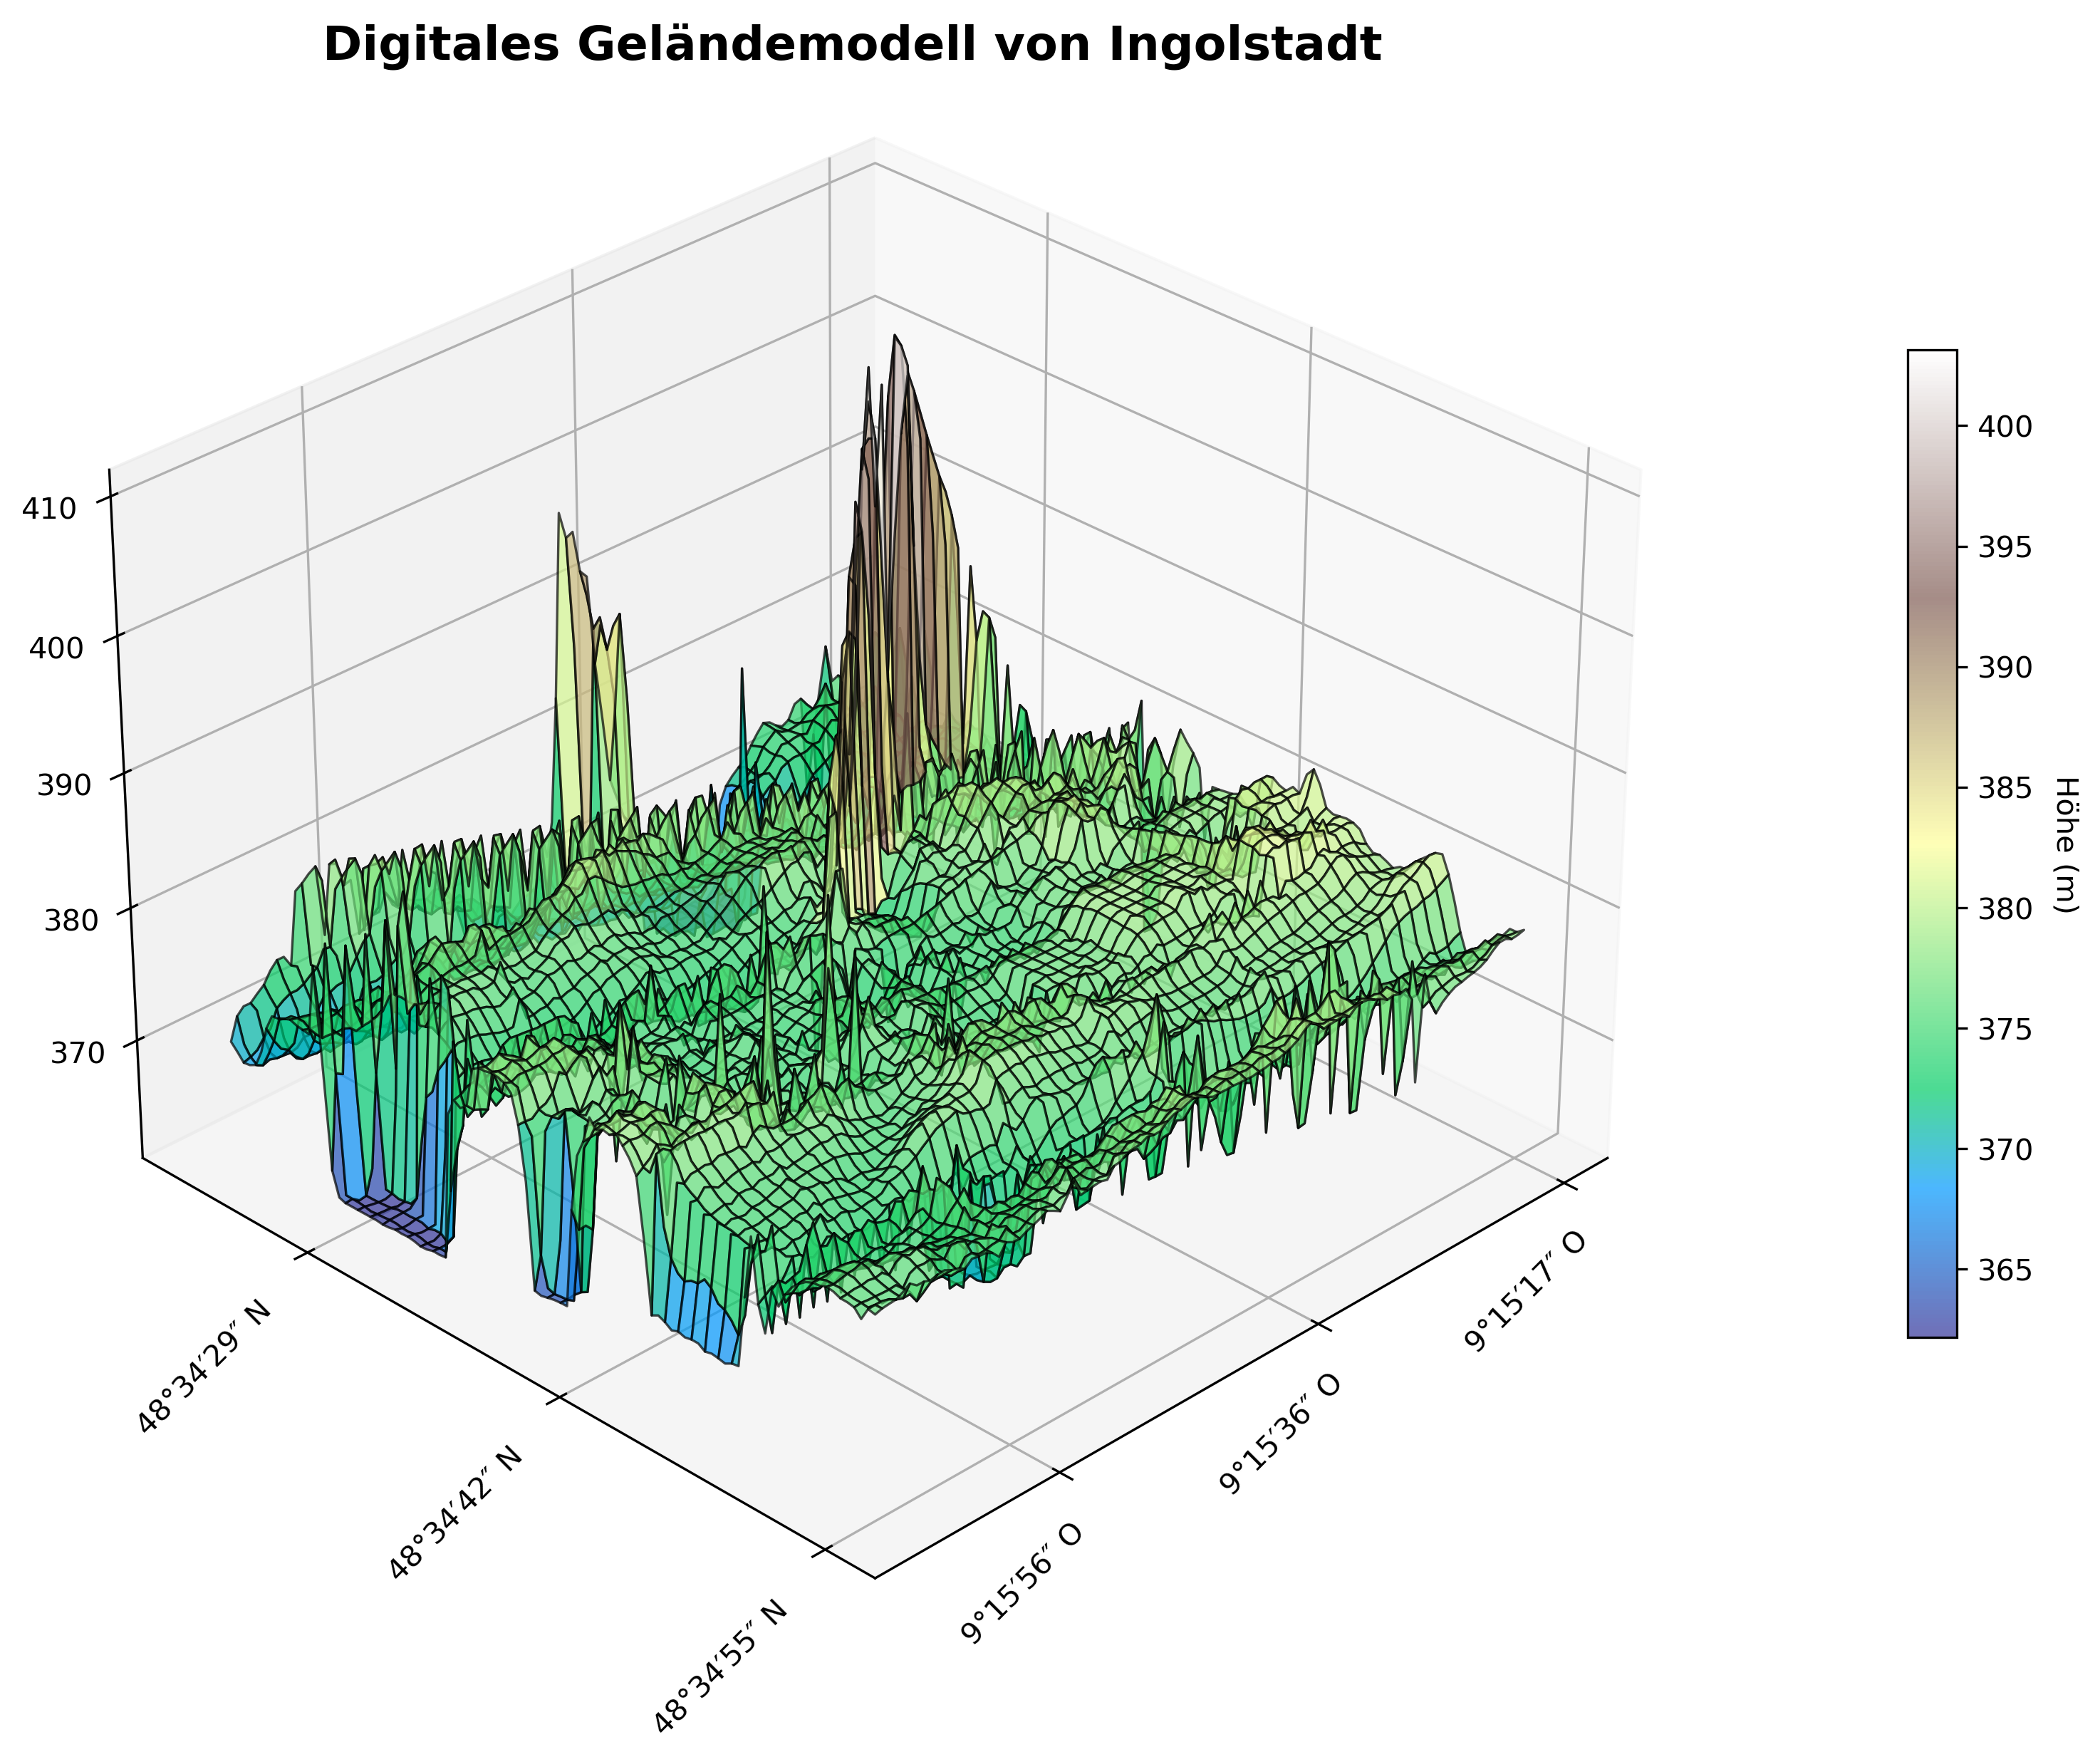
\includegraphics[width=\textwidth]{figures/dgm_3d_wireframe_ingolstadt.png}
    \caption{Digital Geländemodell von Ingolstadt. Quelle: Eigene Darstellung}
    \label{fig:ingolstadt}
\end{figure}
\FloatBarrier